\paragraph{Sơ đồ tuần tự luồng Pha Outbox Relay publish sự kiện mua VIP lên Kafka}

Luồng nghiệp vụ này mô tả

\texttt{OutboxRelayCron} của Payment Service đọc các bản ghi Outbox chưa xử lý, kiểm tra payload của \texttt{SubscriptionPurchasedEvent}, publish sự kiện mua gói VIP lên Kafka thông qua \texttt{MessageBrokerPort}, rồi cập nhật trạng thái Outbox.

\begin{figure}[H]
\centering
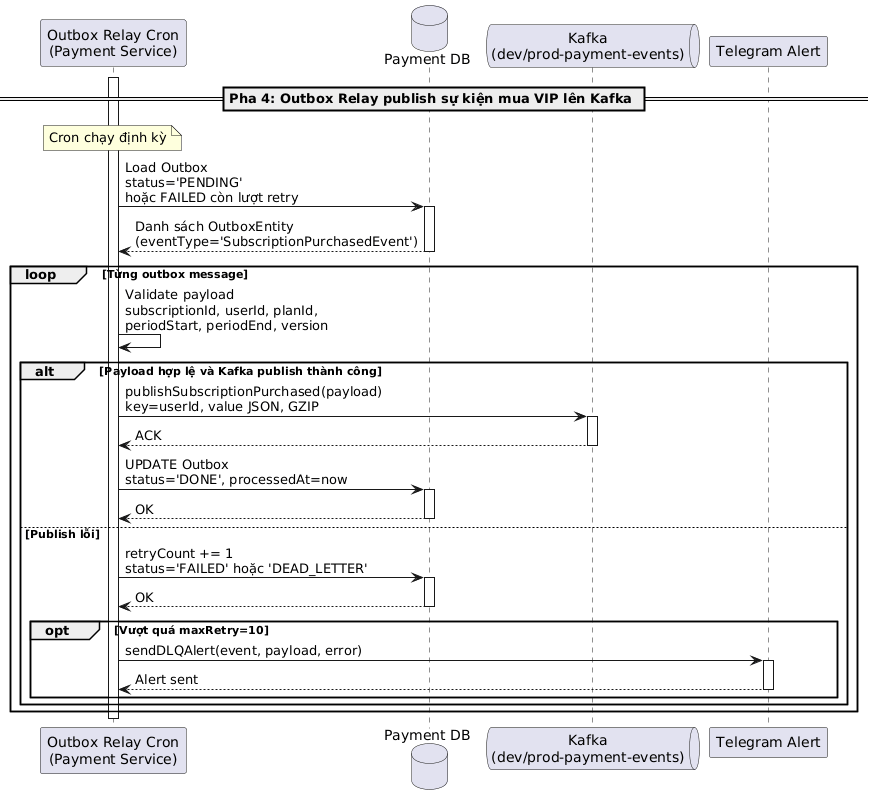
\includegraphics[scale = 0.18]{contents/Sequence/UML-Sequence-PaymentOutboxRelayKafka.png}
\caption{Sơ đồ tuần tự luồng Pha Outbox Relay publish sự kiện mua VIP lên Kafka}
\end{figure}

\subparagraph{Các thành phần tham gia}

\begin{table}[H]
\centering
\renewcommand{\arraystretch}{1.3}
\begin{tabular}{|l|l|p{5cm}|}
\hline
\textbf{Thành phần} & \textbf{Phân loại} & \textbf{Vai trò trong hệ thống} \\ \hline
Outbox Relay Cron & Component & Cron job trong Payment Service, đọc Outbox và điều phối publish sự kiện. \\ \hline
Payment DB & Database & Lưu bảng Outbox với trạng thái \texttt{PENDING}, \texttt{FAILED}, \texttt{DONE} hoặc \texttt{DEAD\_LETTER}. \\ \hline
Kafka & Message Broker & Nhận sự kiện \texttt{SubscriptionPurchased} trên topic \texttt{dev-payment-events} hoặc \texttt{prod-payment-events}. \\ \hline
Telegram Alert & External Service & Nhận cảnh báo khi outbox message vượt quá số lần retry tối đa. \\ \hline
\end{tabular}
\caption{Các thành phần tham gia luồng pha Outbox Relay publish sự kiện mua VIP lên Kafka}
\end{table}

\subparagraph{Mô tả tổng quan}
\begin{itemize}
\item \textbf{Quét Outbox:} Cron định kỳ tải tối đa 50 bản ghi \texttt{PENDING} hoặc \texttt{FAILED} còn lượt retry, có khóa \texttt{pessimistic\_write} và \texttt{skip\_locked}.
\item \textbf{Validate payload:} Với \texttt{SubscriptionPurchasedEvent}, service kiểm tra các trường \texttt{subscriptionId}, \texttt{userId}, \texttt{planId}, \texttt{periodStart}, \texttt{periodEnd}, \texttt{version}.
\item \textbf{Publish Kafka:} Service gọi \texttt{publishSubscriptionPurchased}, Kafka producer gửi message với \texttt{key=userId}, payload JSON và nén GZIP.
\item \textbf{Cập nhật trạng thái:} Nếu publish thành công, Outbox được chuyển sang \texttt{DONE}. Nếu lỗi, service tăng \texttt{retryCount} và chuyển sang \texttt{FAILED}; khi vượt \texttt{maxRetry=10}, chuyển sang \texttt{DEAD\_LETTER} và gửi cảnh báo Telegram.
\end{itemize}
